%!TeX encoding = UTF-8
%!TeX program = xelatex
\documentclass[notheorems, aspectratio=54]{beamer}
% aspectratio: 1610, 149, 54, 43(default), 32

\usepackage{latexsym}
\usepackage{amsmath,amssymb}
\usepackage{mathtools}
\usepackage{color,xcolor}
\usepackage{graphicx}
\usepackage{algorithm}
\usepackage{amsthm}
\usepackage{lmodern} % 解决 font warning
% \usepackage[UTF8]{ctex}
\usepackage{animate} % insert gif

\usepackage{lipsum} % To generate test text 
\usepackage{ulem} % 下划线,波浪线

\usepackage{listings} % display code on slides; don't forget [fragile] option after \begin{frame}
\usepackage{hyperref}
% ----------------------------------------------
% tikx
\usepackage{framed}
\usepackage{tikz}
\usepackage{pgf}
\usetikzlibrary{calc,trees,positioning,arrows,chains,shapes.geometric,%
    decorations.pathreplacing,decorations.pathmorphing,shapes,%
    matrix,shapes.symbols}
\pgfmathsetseed{1} % To have predictable results
% Define a background layer, in which the parchment shape is drawn
\pgfdeclarelayer{background}
\pgfsetlayers{background,main}

% define styles for the normal border and the torn border
\tikzset{
  normal border/.style={black!70!gray, decorate, 
     decoration={random steps, segment length=2.5cm, amplitude=.7mm}},
  torn border/.style={black!70!gray, decorate, 
     decoration={random steps, segment length=.5cm, amplitude=1.7mm}}}

% Macro to draw the shape behind the text, when it fits completly in the
% page
\def\parchmentframe#1{
\tikz{
  \node[inner sep=2em] (A) {#1};  % Draw the text of the node
  \begin{pgfonlayer}{background}  % Draw the shape behind
  \fill[normal border] 
        (A.south east) -- (A.south west) -- 
        (A.north west) -- (A.north east) -- cycle;
  \end{pgfonlayer}}}

% Macro to draw the shape, when the text will continue in next page
\def\parchmentframetop#1{
\tikz{
  \node[inner sep=2em] (A) {#1};    % Draw the text of the node
  \begin{pgfonlayer}{background}    
  \fill[normal border]              % Draw the ``complete shape'' behind
        (A.south east) -- (A.south west) -- 
        (A.north west) -- (A.north east) -- cycle;
  \fill[torn border]                % Add the torn lower border
        ($(A.south east)-(0,.2)$) -- ($(A.south west)-(0,.2)$) -- 
        ($(A.south west)+(0,.2)$) -- ($(A.south east)+(0,.2)$) -- cycle;
  \end{pgfonlayer}}}

% Macro to draw the shape, when the text continues from previous page
\def\parchmentframebottom#1{
\tikz{
  \node[inner sep=2em] (A) {#1};   % Draw the text of the node
  \begin{pgfonlayer}{background}   
  \fill[normal border]             % Draw the ``complete shape'' behind
        (A.south east) -- (A.south west) -- 
        (A.north west) -- (A.north east) -- cycle;
  \fill[torn border]               % Add the torn upper border
        ($(A.north east)-(0,.2)$) -- ($(A.north west)-(0,.2)$) -- 
        ($(A.north west)+(0,.2)$) -- ($(A.north east)+(0,.2)$) -- cycle;
  \end{pgfonlayer}}}

% Macro to draw the shape, when both the text continues from previous page
% and it will continue in next page
\def\parchmentframemiddle#1{
\tikz{
  \node[inner sep=2em] (A) {#1};   % Draw the text of the node
  \begin{pgfonlayer}{background}   
  \fill[normal border]             % Draw the ``complete shape'' behind
        (A.south east) -- (A.south west) -- 
        (A.north west) -- (A.north east) -- cycle;
  \fill[torn border]               % Add the torn lower border
        ($(A.south east)-(0,.2)$) -- ($(A.south west)-(0,.2)$) -- 
        ($(A.south west)+(0,.2)$) -- ($(A.south east)+(0,.2)$) -- cycle;
  \fill[torn border]               % Add the torn upper border
        ($(A.north east)-(0,.2)$) -- ($(A.north west)-(0,.2)$) -- 
        ($(A.north west)+(0,.2)$) -- ($(A.north east)+(0,.2)$) -- cycle;
  \end{pgfonlayer}}}

% Define the environment which puts the frame
% In this case, the environment also accepts an argument with an optional
% title (which defaults to ``Example'', which is typeset in a box overlaid
% on the top border
\newenvironment{parchment}[1][Example]{%
  \def\FrameCommand{\parchmentframe}%
  \def\FirstFrameCommand{\parchmentframetop}%
  \def\LastFrameCommand{\parchmentframebottom}%
  \def\MidFrameCommand{\parchmentframemiddle}%
  \vskip\baselineskip
  \MakeFramed {\FrameRestore}
  \noindent\tikz\node[inner sep=1ex, draw=black!20, fill=black!90, 
          anchor=west, overlay] at (0em, 2em) {\sffamily#1};\par}%
{\endMakeFramed}

% ----------------------------------------------

\mode<presentation>{
    \usetheme{Warsaw}
    % Boadilla CambridgeUS
    % default Antibes Berlin Copenhagen
    % Madrid Montpelier Ilmenau Malmoe
    % Berkeley Singapore Warsaw
    \usecolortheme{seagull}
    % beetle, beaver, orchid, whale, dolphin, seagull
    \useoutertheme{infolines}
    % infolines miniframes shadow sidebar smoothbars smoothtree split tree
    \useinnertheme{circles}
    % circles, rectanges, rounded, inmargin
}

% ---------------------------------------------------------------------
% Jet Black Theme
\setbeamercolor{normal text}{fg=white,bg=black!90}
\setbeamercolor{structure}{fg=white}

\setbeamercolor{alerted text}{fg=red!85!black}

\setbeamercolor{item projected}{use=item,fg=black,bg=item.fg!35}

\setbeamercolor*{palette primary}{use=structure,fg=structure.fg}
\setbeamercolor*{palette secondary}{use=structure,fg=structure.fg!95!black}
\setbeamercolor*{palette tertiary}{use=structure,fg=structure.fg!90!black}
\setbeamercolor*{palette quaternary}{use=structure,fg=structure.fg!95!black,bg=black!80}

\setbeamercolor*{framesubtitle}{fg=white}

\setbeamercolor*{block title}{parent=structure,bg=black!70!gray}
\setbeamercolor*{block body}{fg=black,bg=black!10}
\setbeamercolor*{block title alerted}{parent=alerted text,bg=black!15}
\setbeamercolor*{block title example}{parent=example text,bg=black!15}
% ---------------------------------------------------------------------


% ---------------------------------------------------------------------
% flow chart
\tikzset{
    >=stealth',
    punktchain/.style={
        rectangle, 
        rounded corners, 
        % fill=black!10,
        draw=white, very thick,
        text width=6em,
        minimum height=2em, 
        text centered, 
        on chain
    },
    largepunktchain/.style={
        rectangle,
        rounded corners,
        draw=white, very thick,
        text width=10em,
        minimum height=2em,
        on chain
    },
    line/.style={draw, thick, <-},
    element/.style={
        tape,
        top color=white,
        bottom color=blue!50!black!60!,
        minimum width=6em,
        draw=blue!40!black!90, very thick,
        text width=6em, 
        minimum height=2em, 
        text centered, 
        on chain
    },
    every join/.style={->, thick,shorten >=1pt},
    decoration={brace},
    tuborg/.style={decorate},
    tubnode/.style={midway, right=2pt},
    font={\fontsize{10pt}{12}\selectfont},
}
% ---------------------------------------------------------------------

% code setting
\lstset{
    language=C++,
    basicstyle=\ttfamily\footnotesize,
    keywordstyle=\color{red},
    breaklines=true,
    xleftmargin=2em,
    numbers=left,
    numberstyle=\color[RGB]{222,155,81},
    frame=leftline,
    tabsize=4,
    breakatwhitespace=false,
    showspaces=false,               
    showstringspaces=false,
    showtabs=false,
    morekeywords={Str, Num, List},
}

% ---------------------------------------------------------------------

\newcommand{\reditem}[1]{\setbeamercolor{item}{fg=red}\item #1}

% 缩放公式大小
\newcommand*{\Scale}[2][4]{\scalebox{#1}{\ensuremath{#2}}}

% 解决 font warning
\renewcommand\textbullet{\ensuremath{\bullet}}

% -------------------------------------------------------------

%% preamble
\title[Jet Black Theme]{PPT Template - Jet Black Theme}
% \subtitle{The subtitle}
\author{Roberts}
\institute[]{damon.roberts-1@colorado.edu}

% -------------------------------------------------------------



\title[University of Colorado Boulder]{The new kids are on the block: incentives for House caucuses to disregard seniority in leadership assignments\footnote{Note: Code and Replication data can be found on github: DamonCharlesRoberts/seniority-project}}
\author[\copyright\ Roberts 2020]{
Damon C. Roberts\\ \bigskip 
{\small University of Colorado Boulder} } 
\date{12/10/2020}

\begin{document}

\frame{\titlepage}


%----------------What we are doing today slide
\begin{frame}\frametitle{The Puzzle}
	\begin{itemize}\setlength\itemsep{1em}
		\item Scholars propose that the (now) informal seniority system works as a useful heuristic for the caucus to elect more senior members in the House (see Taylor, 2019)
			\begin{itemize}
				\item This has a number of assumptions tied to it
			\end{itemize}
		\item This project seeks to determine under what circumstances may it be beneficial for the caucus to replace incumbents in leadership positions with less senior MC's.
	\end{itemize}	
\end{frame}

\begin{frame}\frametitle{What the literature says}
	\begin{itemize}\setlength\itemsep{1em}
		\item First, what do other caucuses look like in Congress?
	\end{itemize}
\end{frame}

\begin{frame}\frametitle{What the literature says}
	\begin{itemize}\setlength\itemsep{1em}
		\item First, what do other caucuses look like in Congress?
		\begin{itemize}
			\item Some had argued that parties mattered very little in shaping MC behavior (Mayhew 1974; Aldrich 1995,2011; Krehbiel 1991)
		\end{itemize}
	\end{itemize}
\end{frame}

\begin{frame}\frametitle{What the literature says}
	\begin{itemize}\setlength\itemsep{1em}
		\item First, what do other caucuses look like in Congress?
		\begin{itemize}
			\item Some had argued that parties mattered very little in shaping MC behavior (Mayhew 1974; Aldrich 1995,2011; Krehbiel 1991)
			\item Others have argued that parties are more powerful (Rohde 1991; Cox and McCubbins 2005)
		\end{itemize}
	\end{itemize}
\end{frame}

\begin{frame}\frametitle{What the literature says}
	\begin{itemize}\setlength\itemsep{1em}
		\item Second, what are the driving motivations for MC's
	\end{itemize}
\end{frame}

\begin{frame}\frametitle{What the literature says}
	\begin{itemize}\setlength\itemsep{1em}
		\item Second, what are the driving motivations for MC's
		\begin{itemize}
			\item Fenno says that they have three goals
		\end{itemize}
	\end{itemize}
\end{frame}

\begin{frame}\frametitle{What the literature says}
	\begin{itemize}\setlength\itemsep{1em}
		\item Second, what are the driving motivations for MC's
		\begin{itemize}
			\item Fenno says that they have three goals
			\begin{itemize}
				\item Reelection
				\item Achieve more power/influence
				\item Good public policy
			\end{itemize}
		\end{itemize}
	\end{itemize}
\end{frame}

\begin{frame}\frametitle{What the literature says}
	\begin{itemize}\setlength\itemsep{1em}
		\item Second, what are the driving motivations for MC's
		\begin{itemize}
			\item Fenno says that they have three goals
			\begin{itemize}
				\item Reelection
				\item Achieve more power/influence
				\item Good public policy
			\end{itemize}
			\item Mayhew states that they are primarily concerned with reelection
			\item The caucus has goals to ensure that they retain majority status
		\end{itemize}
	\end{itemize}
\end{frame}

\begin{frame}\frametitle{Adjusting motivations}
	\begin{equation} 
		C_\beta = \DeclareMathOperator{argMax}{(\beta_i)}
	\end{equation}
	\begin{equation}
		i_\beta = \DeclareMathOperator{argMin}{(\beta_i)}
	\end{equation}
\end{frame}

\begin{frame}\frametitle{Adjusting motivations}
	\begin{equation} \label{eq:3}
		\prod \DeclareMathOperator{argMax}{(\beta_i)} > \prod \DeclareMathOperator{argMin}{\beta_i}	
	\equiv
	C_\beta > i_\beta
	\end{equation}
	\begin{equation} \label{eq:4}
	\prod \DeclareMathOperator{argMax}{(\beta_i)} \approx \prod \DeclareMathOperator{argMin}{\beta_i}
	\equiv
	C_\beta \approx i_\beta
\end{equation}
\end{frame}

\begin{frame}\frametitle{Adjusting motivations}
	\begin{equation} \label{eq:5}
	m_\beta = \DeclareMathOperator{argMin}{(\beta)}
\end{equation} 

\begin{equation} \label{eq:6}
	\prod\DeclareMathOperator{argMax}{(\beta_m)} \approx \prod\DeclareMathOperator{argMin}{(\beta_m)}
	\equiv
	C_\beta \approx m_\beta
\end{equation}
\end{frame}

\begin{frame}\frametitle{The Game}
	\begin{center}
	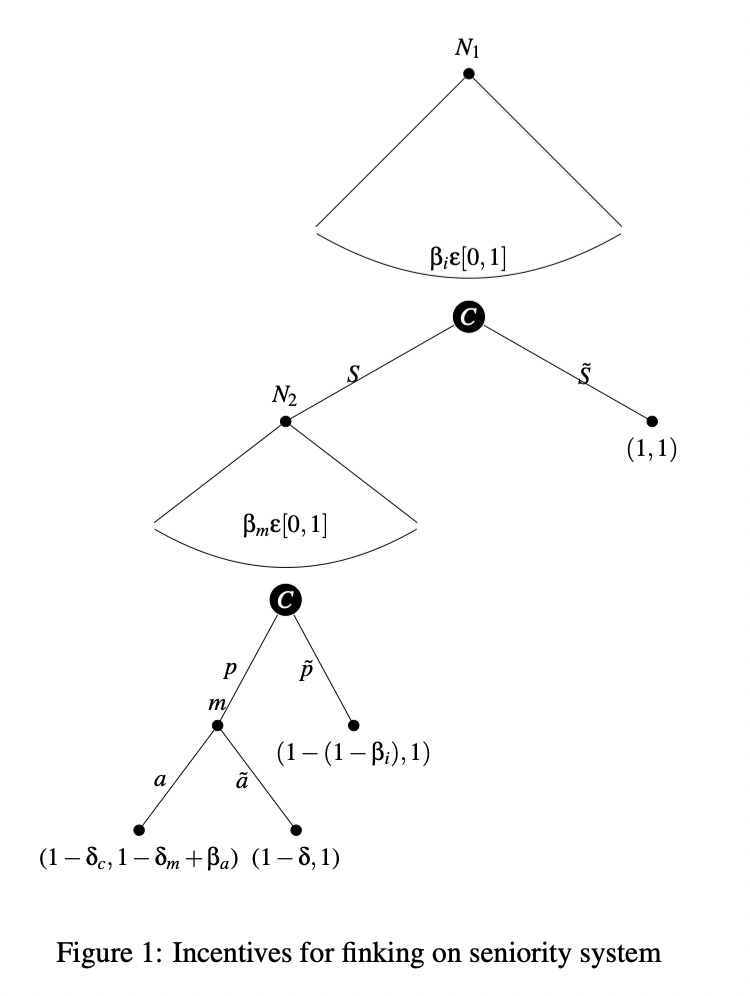
\includegraphics[height=75mm, width=75mm]{fig1-updated}
	\end{center}
\end{frame}
\begin{frame}\frametitle{Descriptive empirics}
	\begin{center}
		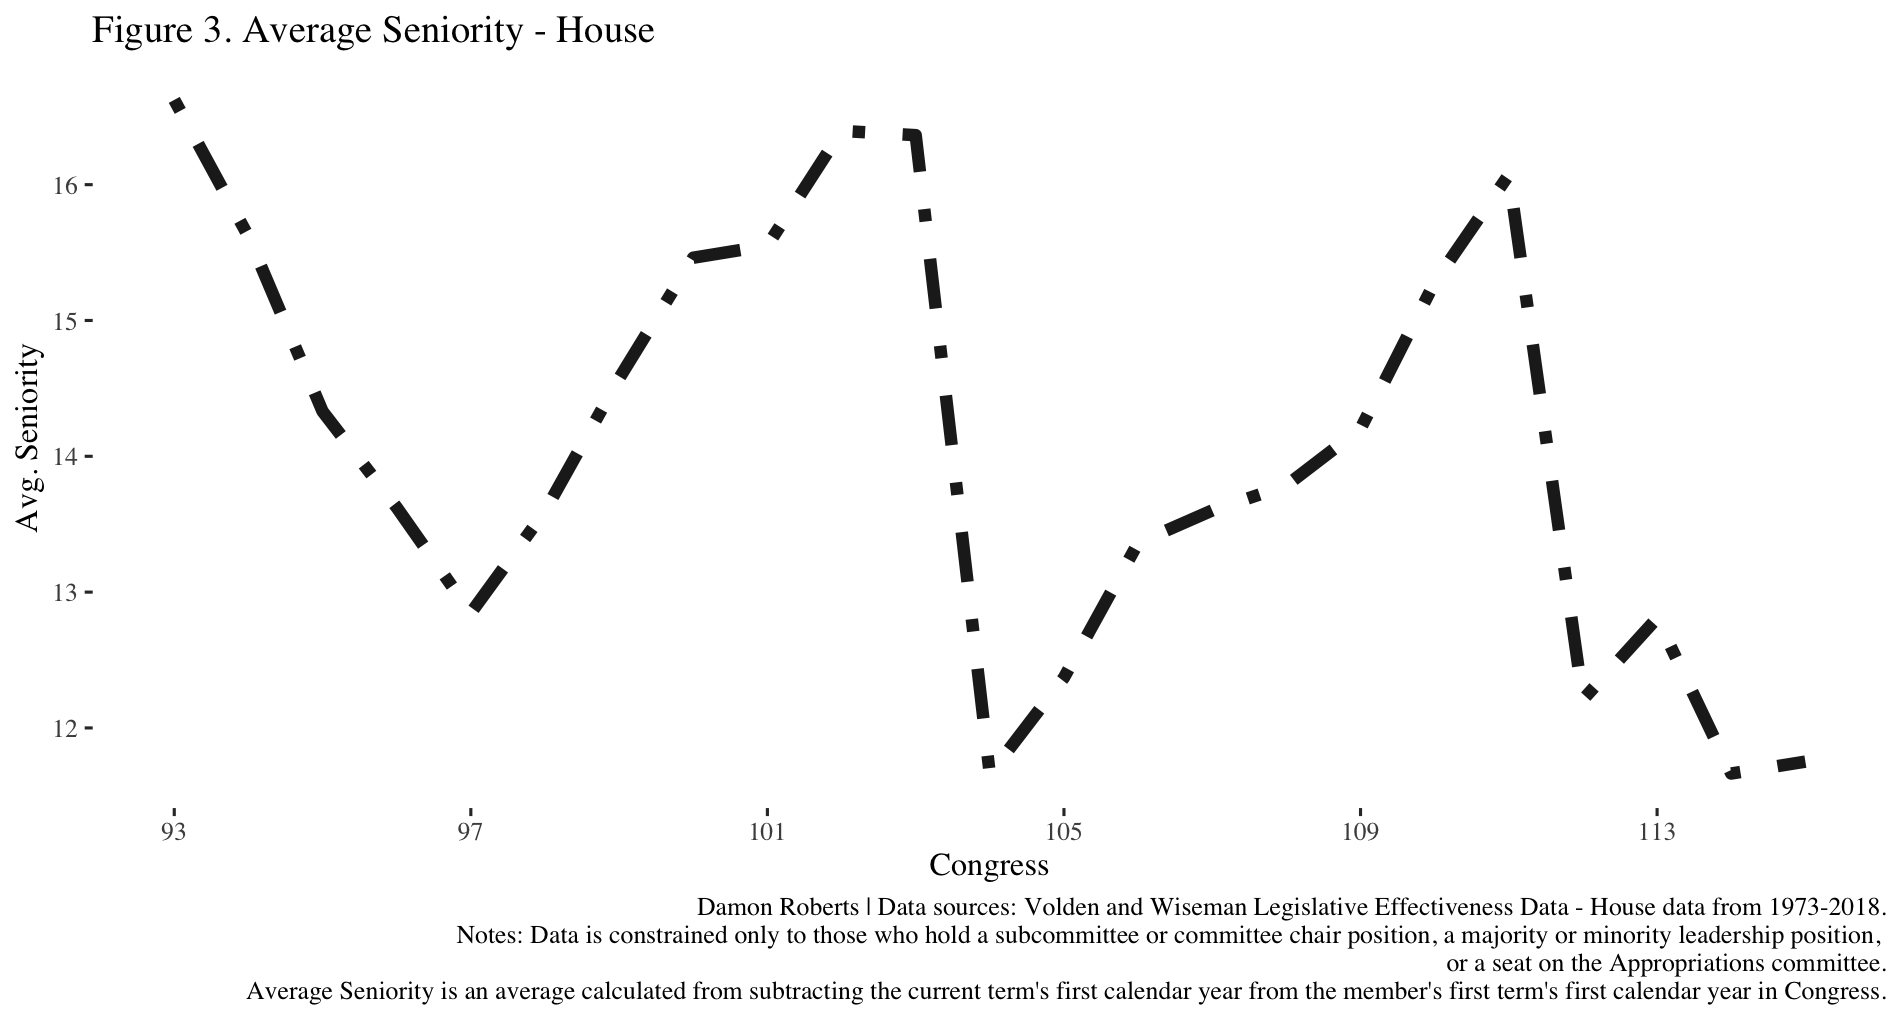
\includegraphics[height=75mm,width=75mm]{../figures/avg-house-seniority-macro}
	\end{center}
\end{frame}

\begin{frame}\frametitle{Questions/Comments?}
	
\end{frame}
\end{document}